\documentclass[11pt]{article}

\usepackage[margin=1in]{geometry}
\usepackage{amsfonts, amsmath, amssymb}
\usepackage{fancyhdr, float, graphicx}
\usepackage[utf8]{inputenc} % Required for inputting international characters
\usepackage[T1]{fontenc} % Output font encoding for international characters
\usepackage{fouriernc} % Use the New Century Schoolbook font
\usepackage[nottoc, notlot, notlof]{tocbibind}
\usepackage{listings}
\usepackage{xcolor}
\usepackage{blindtext}
\usepackage{hyperref}
\hypersetup{
	colorlinks=true,
	linkcolor=black,
	filecolor=magenta,
	urlcolor=blue,
	pdfpagemode=FullScreen,
}

\definecolor{codegreen}{rgb}{0,0.6,0}
\definecolor{codegray}{rgb}{0.5,0.5,0.5}
\definecolor{codepurple}{rgb}{0.58,0,0.82}
\definecolor{backcolour}{rgb}{0.95,0.95,0.92}

\lstdefinestyle{mystyle}{
	backgroundcolor=\color{backcolour},
	commentstyle=\color{codegreen},
	keywordstyle=\color{magenta},
	numberstyle=\tiny\color{codegray},
	stringstyle=\color{codepurple},
	basicstyle=\ttfamily\footnotesize,
	breakatwhitespace=false,
	breaklines=true,
	captionpos=b,
	keepspaces=true,
	numbers=left,
	numbersep=5pt,
	showspaces=false,
	showstringspaces=false,
	showtabs=false,
	tabsize=2
}

\lstset{style=mystyle}

% Header and Footer
\pagestyle{fancy}
\fancyhead{}
\fancyfoot{}
\fancyhead[L]{\textit{\Large{Attack Reserach and Documentation - Fourth Year B. Tech}}}
\fancyhead[R]{\textit{Krishnaraj T}}
\fancyfoot[C]{\thepage}
\renewcommand{\footrulewidth}{1pt}

\begin{document}

\begin{titlepage}
	\centering

	%---------------------------NAMES-------------------------------

	\huge\textsc{
		MIT World Peace University
	}\\

	\vspace{0.75\baselineskip} % space after Uni Name

	\LARGE{
		Attack Research and Documentation\\
		Fourth Year B. Tech, Semester 5
	}

	\vfill % space after Sub Name

	%--------------------------TITLE-------------------------------

	\rule{\textwidth}{1.6pt}\vspace*{-\baselineskip}\vspace*{2pt}
	\rule{\textwidth}{0.6pt}
	\vspace{0.75\baselineskip} % Whitespace above the title

	\huge{\textsc{
        Study of Various Tools for Simulated
            Attack Scenarioss
        }} \\

	\vspace{0.5\baselineskip} % Whitespace below the title
	\rule{\textwidth}{0.6pt}\vspace*{-\baselineskip}\vspace*{2.8pt}
	\rule{\textwidth}{1.6pt}

	\vspace{1\baselineskip} % Whitespace after the title block

	%--------------------------SUBTITLE --------------------------	

	\LARGE\textsc{
		Lab Assignment 1 Report
	} % Subtitle or further description
	\vfill

	%--------------------------AUTHOR-------------------------------

	Prepared By \vspace{0.5\baselineskip} % Whitespace before the editors

	\Large{
		Krishnaraj Thadesar \\
		Cyber Security and Forensics\\
        Batch A1, PA 15
	}

	\vspace{0.5\baselineskip} % Whitespace below the editor list
	\today

\end{titlepage}

\tableofcontents
\thispagestyle{empty}
\clearpage

\setcounter{page}{1}

\section{Aim}
To study and document the working of various tools used for simulated attack scenarios.

\section{Wireshark}

\begin{figure}[H]
	\centering
	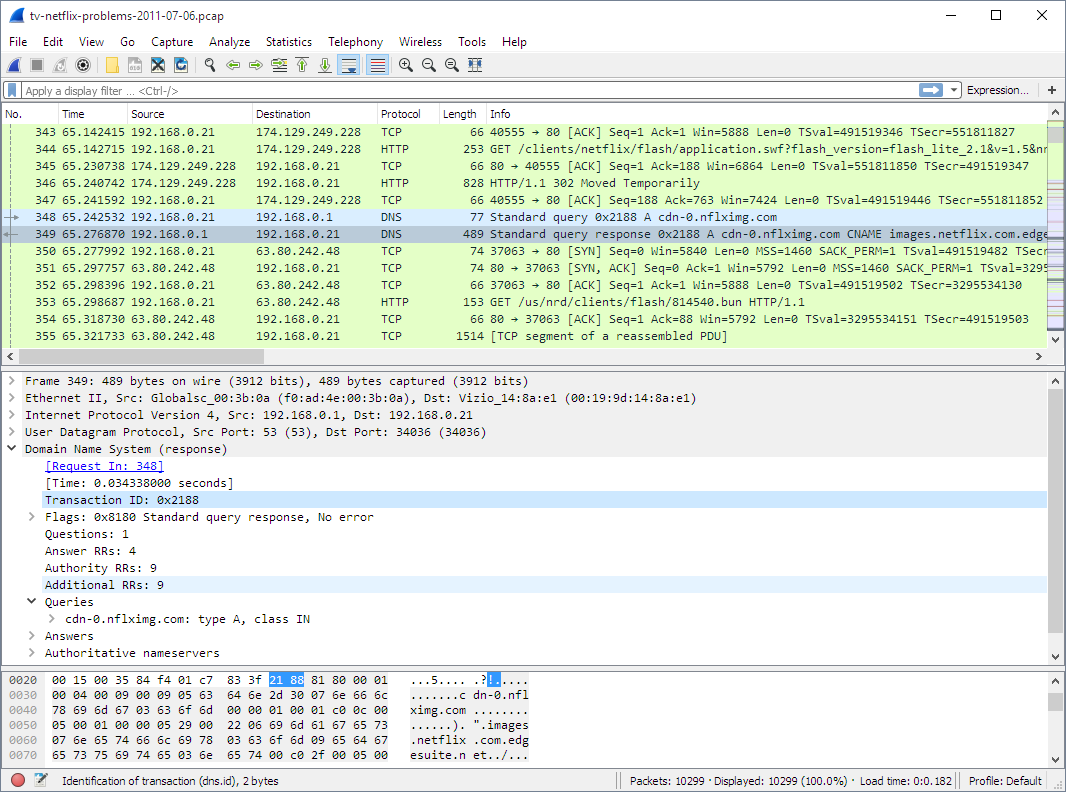
\includegraphics[width=.95\textwidth]{img/wireshark/wireshark_0.jpg}
	\caption{Wireshark GUI}
\end{figure}

\subsection{Installation}
\begin{itemize}
	\item \textbf{Procedure:} Wireshark can be installed on various operating systems, including Windows, macOS, and Linux. Visit the official Wireshark website (\url{https://www.wireshark.org/}) and follow the installation instructions for your specific platform.
	\item \textbf{Dependencies:} Wireshark may require the installation of WinPcap (Windows), libpcap (Linux), or npcap (Windows) for packet capture.
\end{itemize}

\subsection{Working}
\begin{itemize}
	\item Wireshark captures and analyzes packets on a network in real-time.
	\item Users can apply various filters to focus on specific types of traffic.
	\item The captured data can be displayed in different formats, facilitating detailed
	      protocol analysis.
\end{itemize}

\subsection{Pros}
\begin{itemize}
	\item User-friendly interface with powerful features.
	\item Extensive protocol support for in-depth analysis.
	\item Active community and regular updates.
\end{itemize}

\subsection{Cons}
\begin{itemize}
	\item May consume significant system resources during packet capture.
	\item Beginners might find the wealth of features overwhelming.
	\item Limited to the capabilities of the network interface card (NIC).
\end{itemize}

\subsection{Using Wireshark to Capture Packet and get password details. }

\begin{figure}[H]
    \centering
    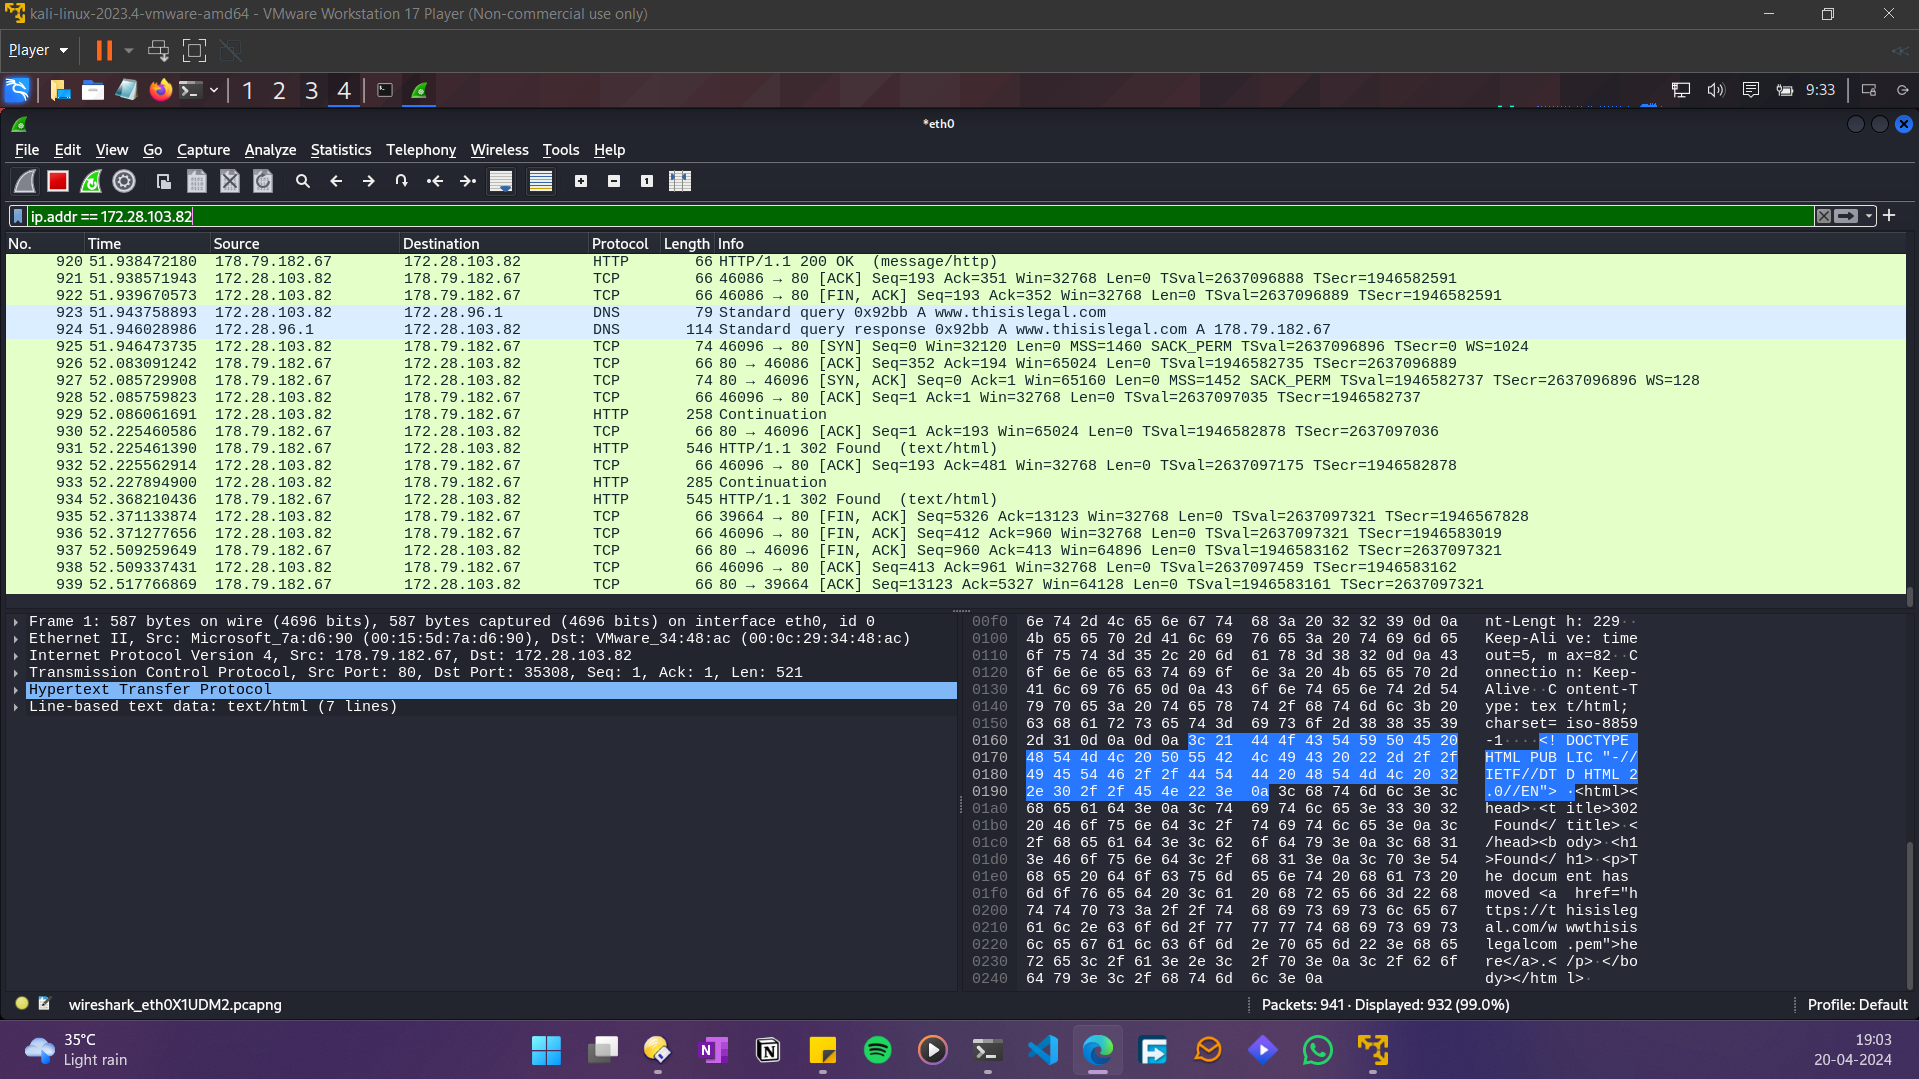
\includegraphics[width=0.99\textwidth]{assignment 8 (1).png}
    \caption{Filtering by target ip}
\end{figure}
\begin{figure}[H]
    \centering
    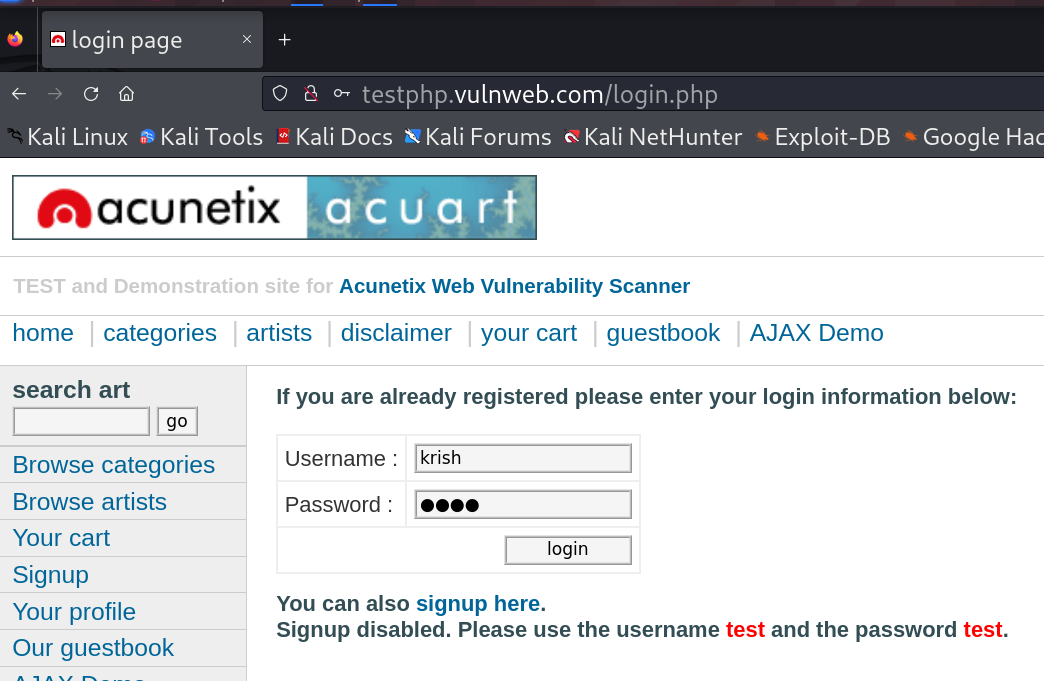
\includegraphics[width=0.99\textwidth]{assignment 8 (3).png}
    \caption{Login Request from ip}
\end{figure}

\begin{figure}[H]
    \centering
    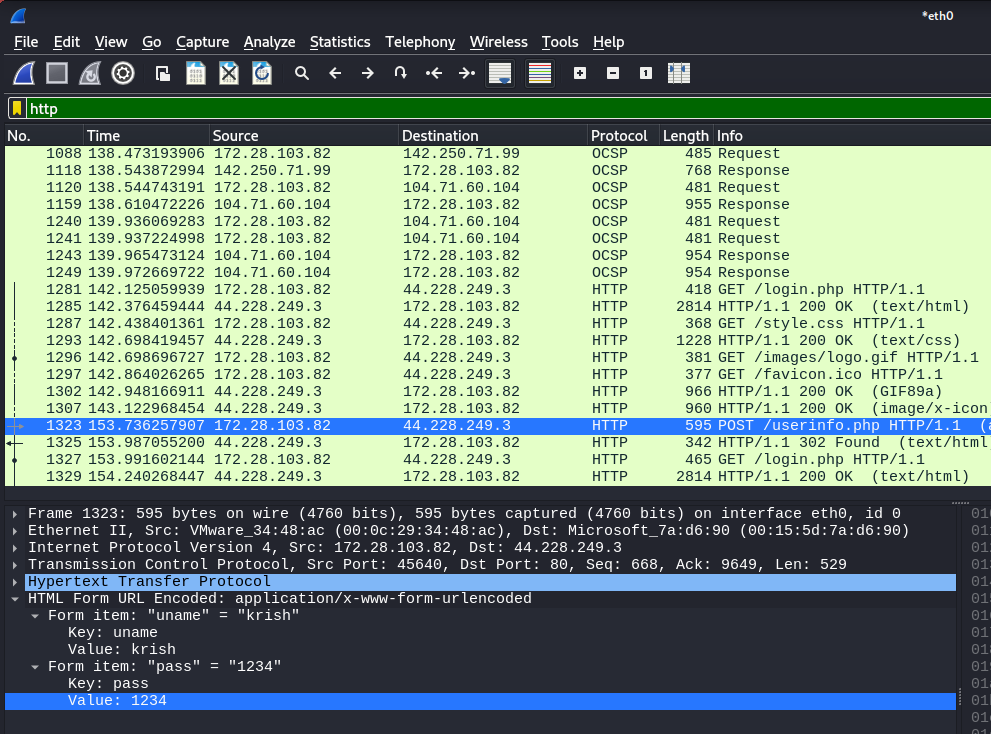
\includegraphics[width=0.99\textwidth]{assignment 8 (2).png}
    \caption{Viewing Http packets to get username and password}
\end{figure}


\begin{figure}[H]
	\centering
	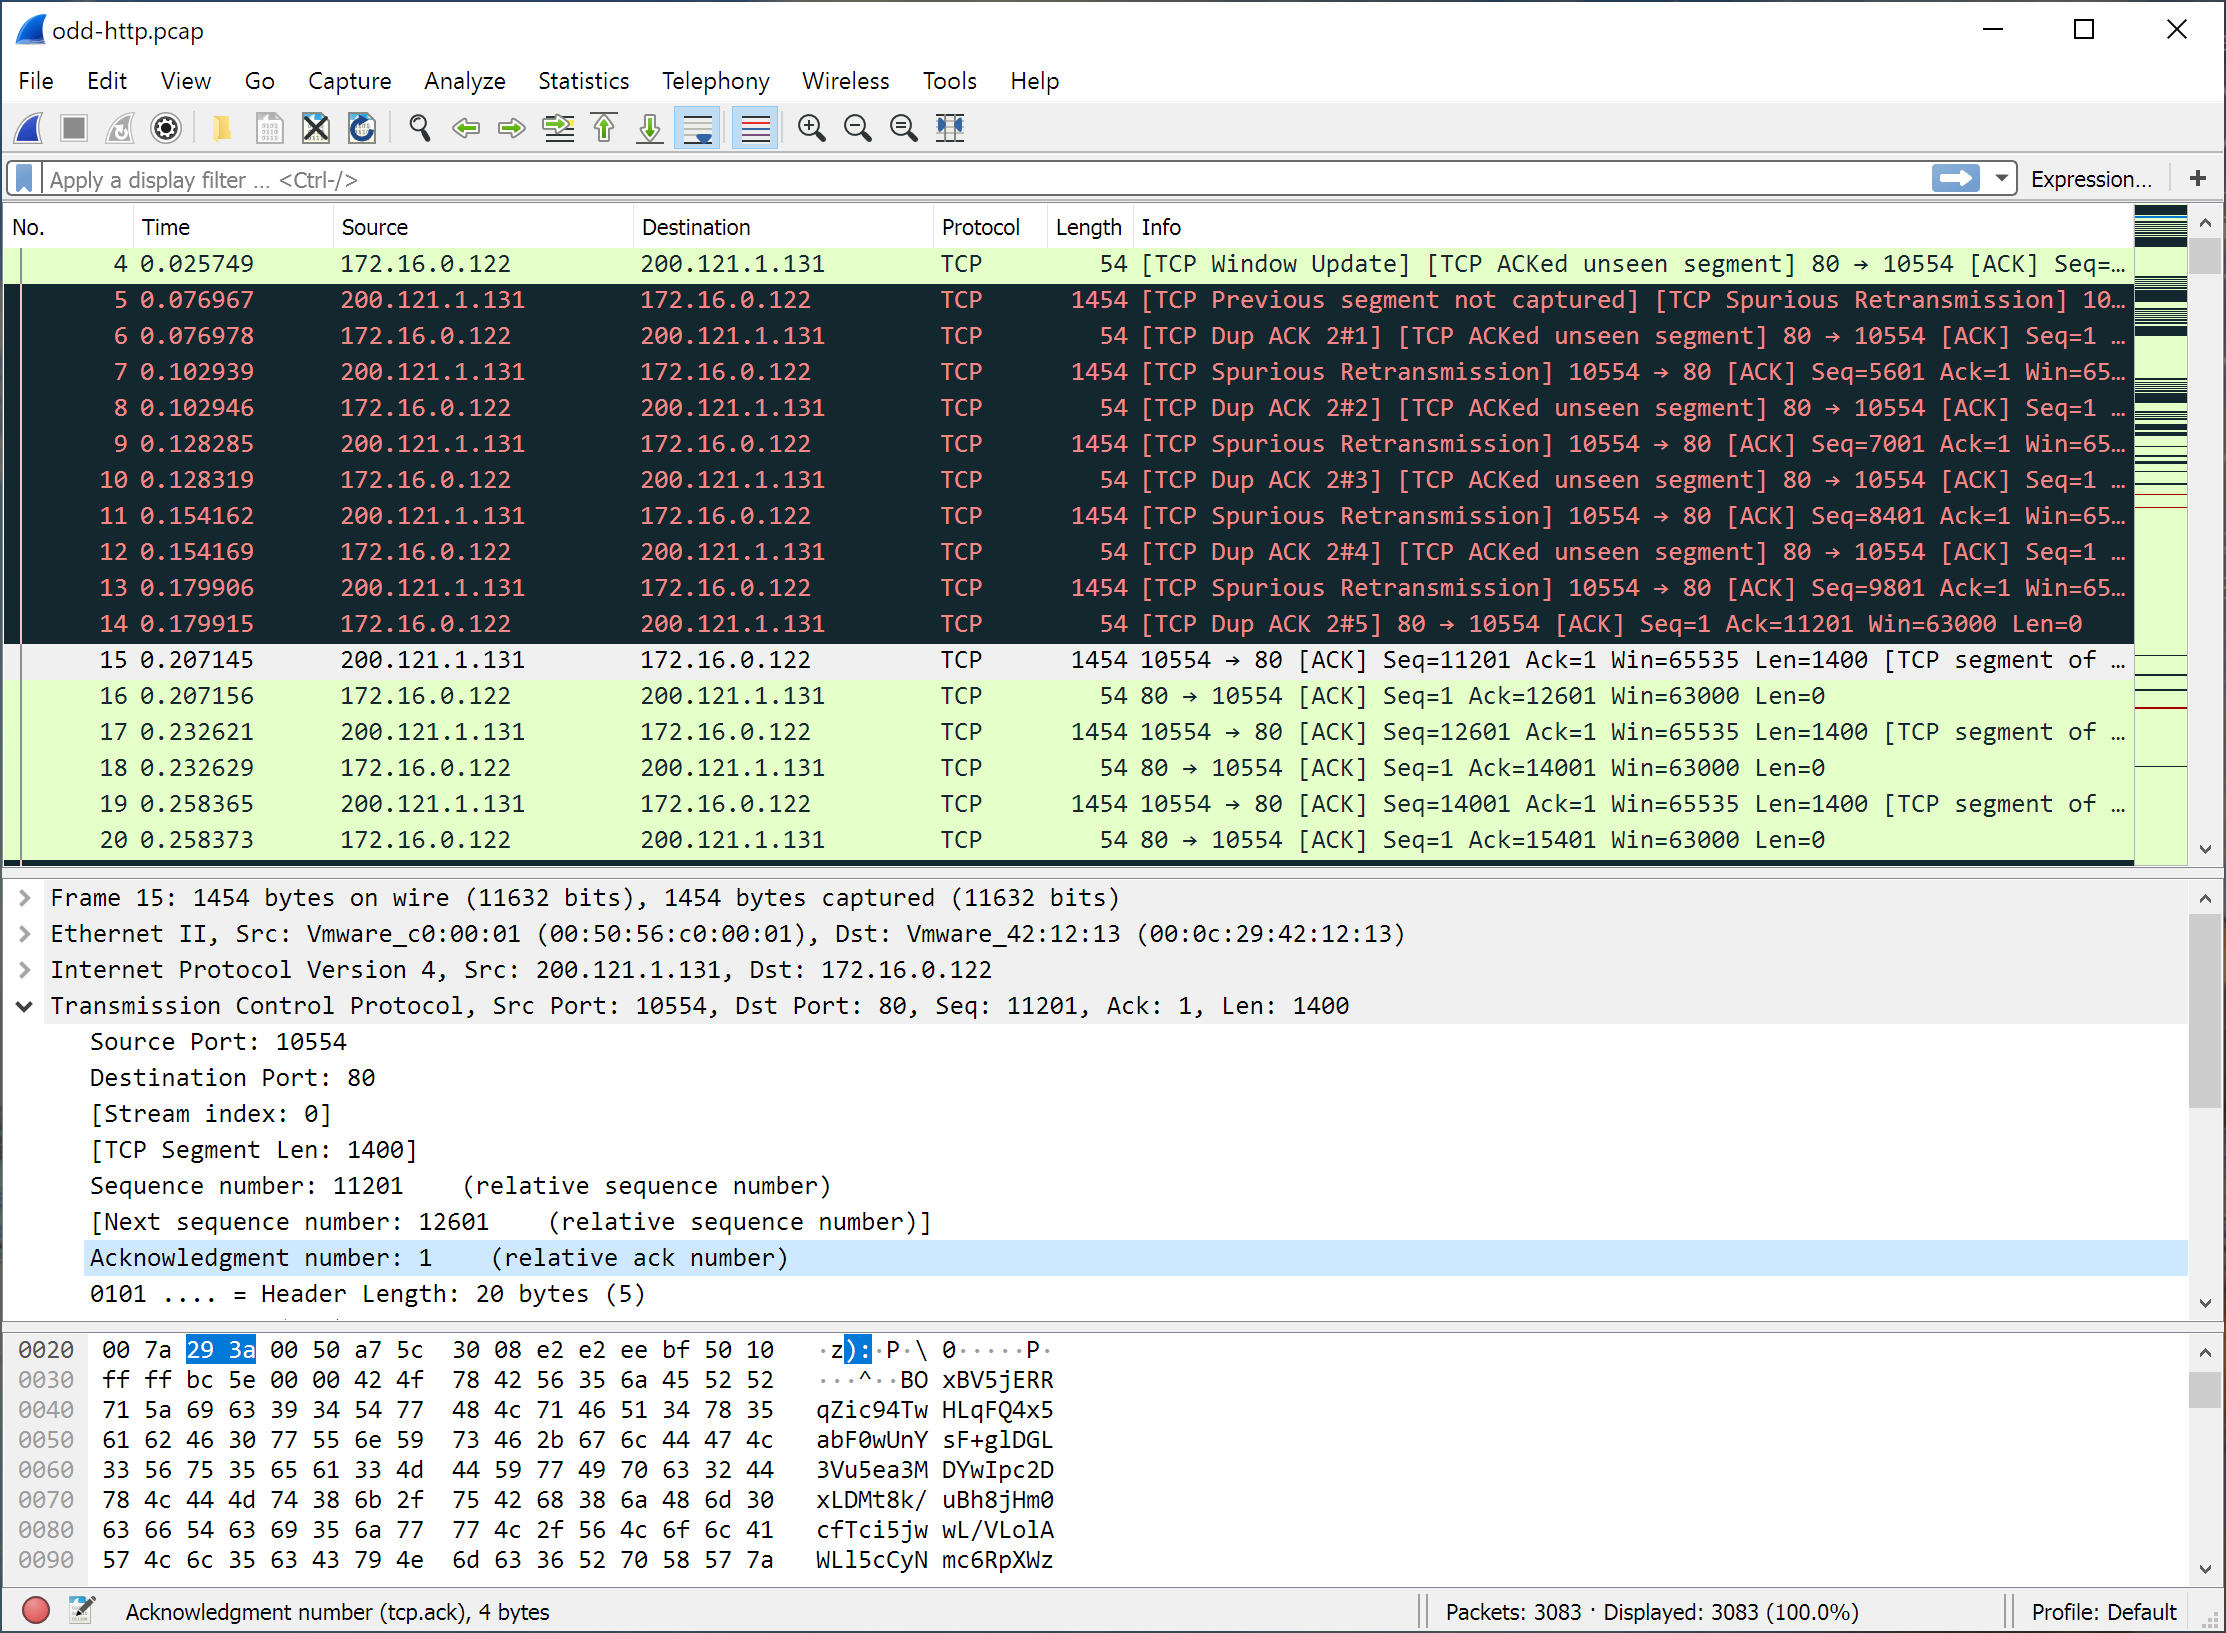
\includegraphics[width=.95\textwidth]{img/wireshark/wireshark_8.jpg}
	\caption{A command-line window executing the aireplay-ng-death tool to deauthenticate clients from a Wi-Fi network. }
\end{figure}

\begin{figure}[H]
	\centering
	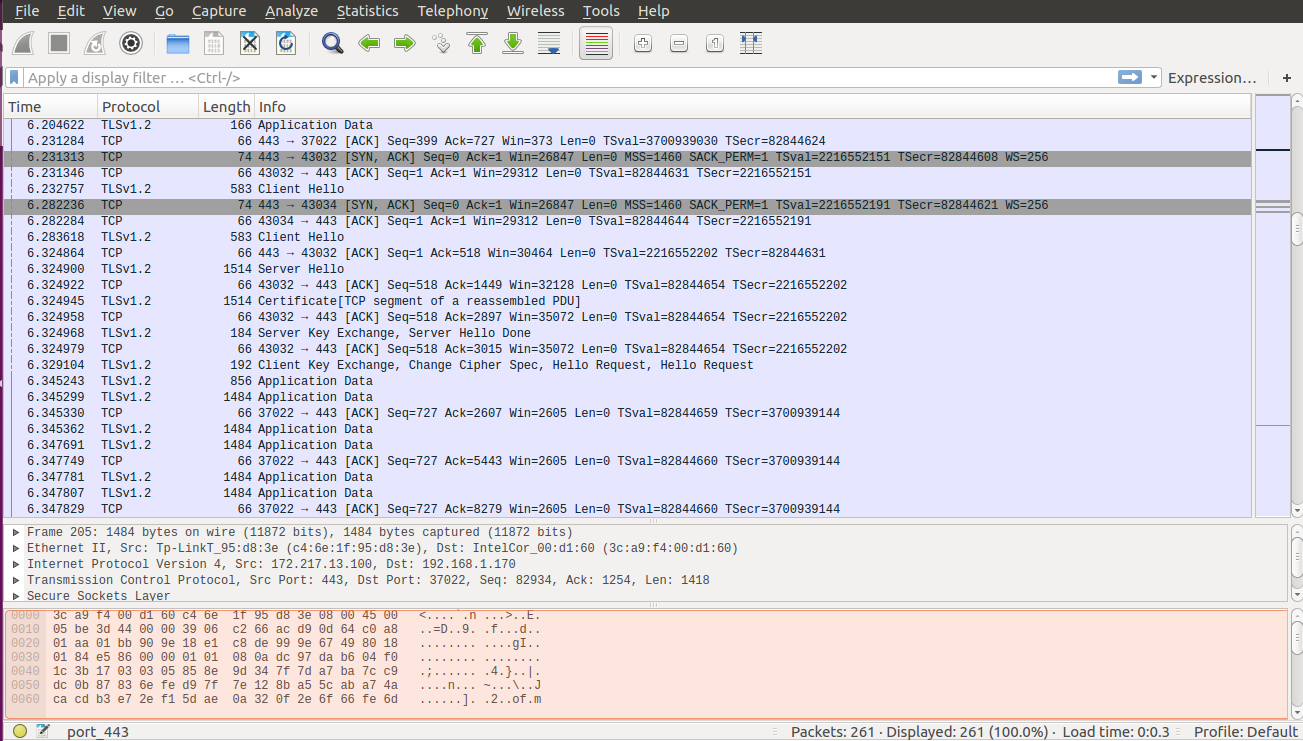
\includegraphics[width=.95\textwidth]{img/wireshark/wireshark_9.jpg}
	\caption{Wi-Fi network scan results on a Kali Linux system.	}
\end{figure}

\section{Nmap}
Nmap, short for Network Mapper, is a widely-used open-source tool designed for network exploration and security auditing. It provides a comprehensive view of a network by discovering hosts and services running on them.

\subsection{Need/Purpose of Nmap}
Nmap serves various purposes in the field of cybersecurity and network management. Its primary objectives include:

\begin{itemize}
    \item \textbf{Host Discovery:} Identifying active hosts on a network, aiding in network mapping.
    \item \textbf{Port Scanning:} Determining open ports on a system, crucial for understanding potential vulnerabilities.
    \item \textbf{Service Version Detection:} Identifying the version and type of services running on open ports.
    \item \textbf{OS Fingerprinting:} Attempting to determine the operating system of target hosts.
    \item \textbf{Vulnerability Assessment:} Assessing potential security risks and vulnerabilities within a network.
\end{itemize}

\subsection{Advantages of Nmap}
Nmap offers several advantages that make it a preferred choice in the cybersecurity community:

\begin{itemize}
    \item \textbf{Versatility:} Nmap can be used for a wide range of network exploration and security auditing tasks.
    \item \textbf{Accuracy:} It provides accurate information about hosts, open ports, and services.
    \item \textbf{Scripting Engine:} Nmap's scripting engine allows users to create custom scripts for specific tasks.
    \item \textbf{Community Support:} Being open-source, Nmap benefits from a large and active user community, ensuring continuous improvement.
    \item \textbf{Platform Independence:} Nmap is available on multiple platforms, making it accessible to a diverse range of users.
\end{itemize}

\subsection{Disadvantages of Nmap}
Despite its many strengths, Nmap has some limitations and potential drawbacks:

\begin{itemize}
    \item \textbf{Firewall Interference:} Firewalls may block Nmap scans, limiting the tool's effectiveness.
    \item \textbf{Legal and Ethical Concerns:} Improper use of Nmap for unauthorized scanning may lead to legal and ethical issues.
    \item \textbf{False Positives:} In certain scenarios, Nmap might produce false positives, leading to inaccurate assessments.
    \item \textbf{Resource Intensive:} Intensive scanning can consume significant network resources and slow down target systems.
    \item \textbf{Limited Stealth:} While Nmap offers stealthy scanning options, complete stealth is challenging to achieve in some situations.
\end{itemize}

\subsection{Implementation}

\subsection{Get ip Address}

\subsubsection*{Syntax}
\begin{verbatim}
$ifconfig
\end{verbatim}

\subsubsection*{Command}
\begin{verbatim}
$ifconfig
\end{verbatim}

\subsubsection*{Purpose}
To get the IP Address of the machine.

\subsubsection*{Output}
\begin{figure}[H]
    \centering
    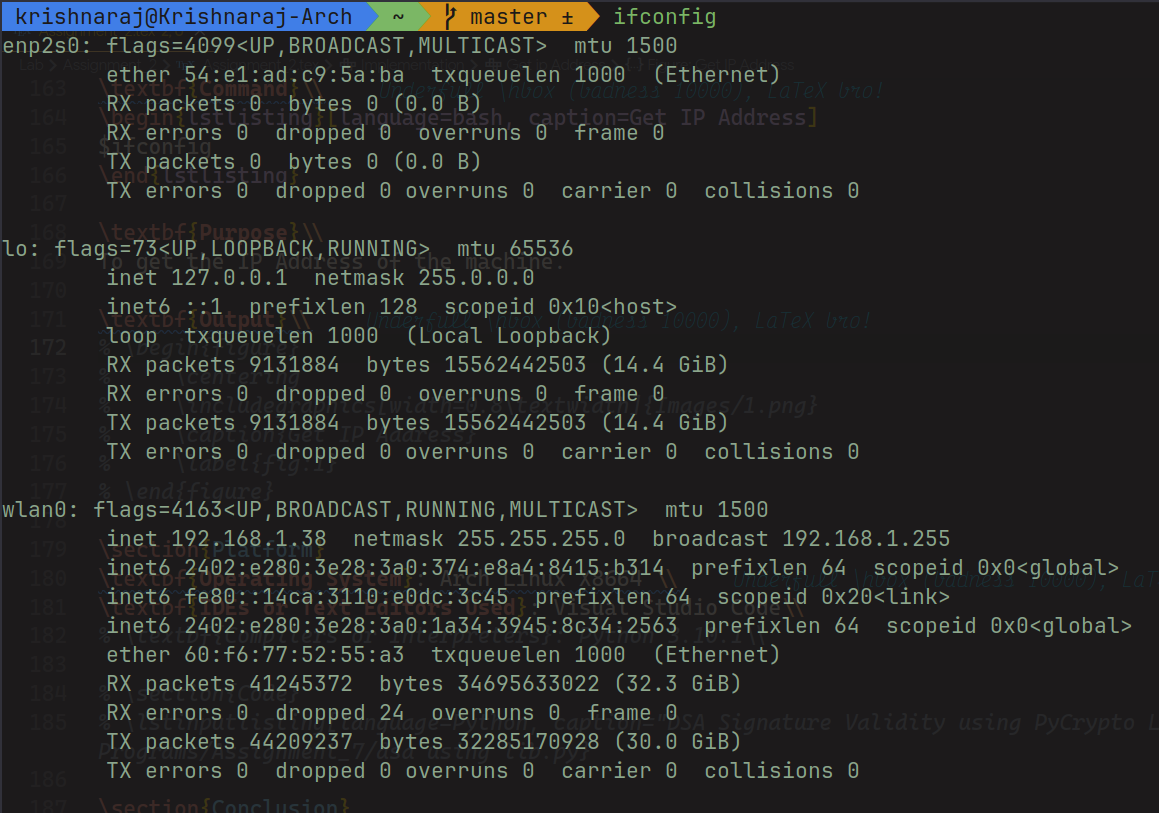
\includegraphics[width=0.8\textwidth]{ifconfig.png}
    \caption{Get IP Address}
    \label{fig:1}
\end{figure}

\subsection{Scan 1 port, current IP}

\subsubsection{Syntax}
\begin{verbatim}
$ nmap -p <port> <ip>
\end{verbatim}

\subsubsection*{Command}
\begin{verbatim}
$ nmap -p 80 192.168.1.38
\end{verbatim}

\subsubsection*{Purpose}
To get the IP Address of the machine.

\subsubsection*{Output}
\begin{figure}[H]
    \centering
    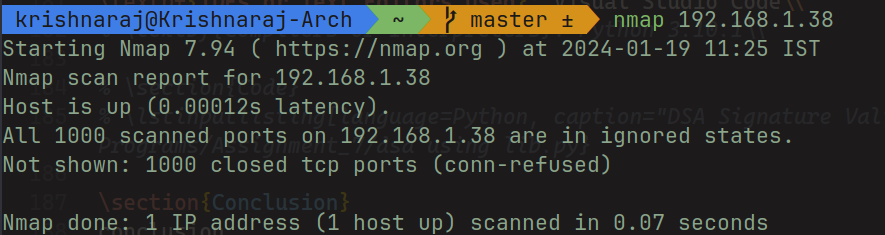
\includegraphics[width=0.8\textwidth]{nmap ip.png}
    \caption{Get IP Address}
    \label{fig:1}
\end{figure}

\subsection{Scan any IP}

\subsubsection{Syntax}
\begin{verbatim}
$ nmap <ip>
\end{verbatim}

\subsubsection*{Command}
\begin{verbatim}
$ nmap 192.168.1.38
\end{verbatim}

\subsubsection*{Purpose}
Scan a single ip

\subsubsection*{Output}
\begin{figure}[H]
    \centering
    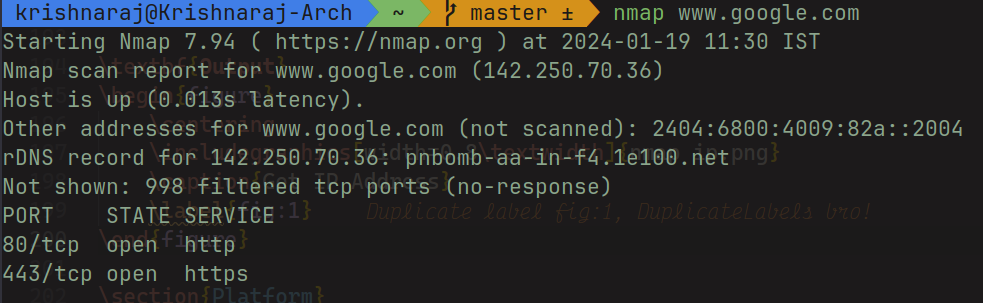
\includegraphics[width=0.8\textwidth]{nmap google.png}
    \caption{Scan google.com}
    \label{fig:1}
\end{figure}

\subsection{Scan a range of IPs}

\subsubsection{Syntax}
\begin{verbatim}
$ nmap <ip range>
\end{verbatim}

\subsubsection*{Command}
\begin{verbatim}
$ nmap 192.168.1.38-40
\end{verbatim}

\subsubsection*{Purpose}
To Scan a range of IPs.

\subsubsection*{Output}
\begin{figure}[H]
    \centering
    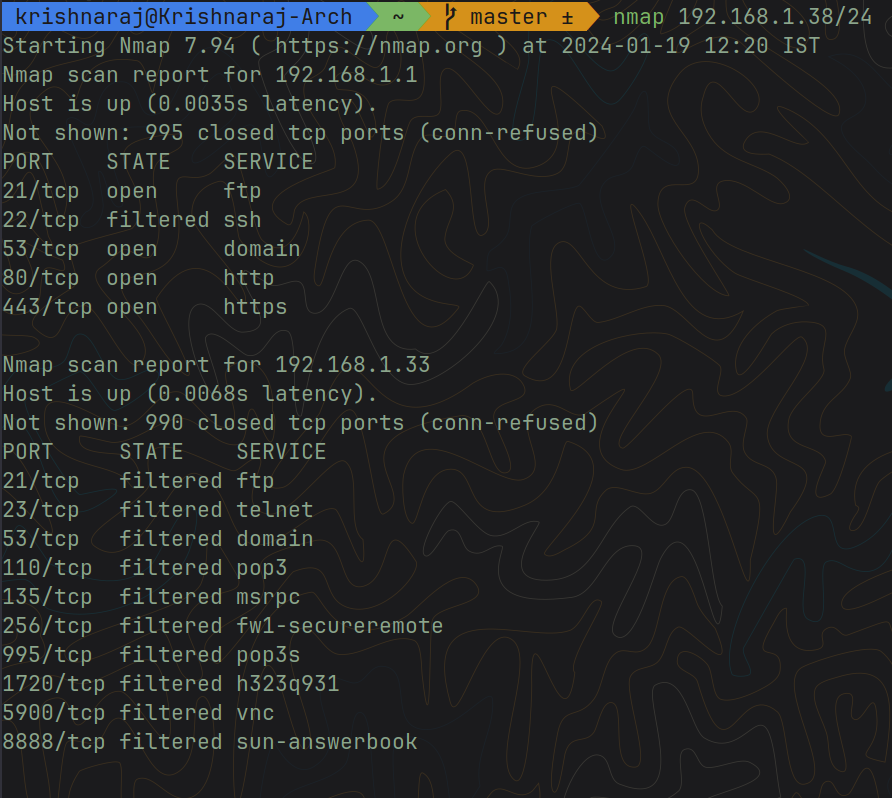
\includegraphics[width=0.8\textwidth]{scan ip range 1.png}
    \caption{scan range of ips. }
    \label{fig:1}
\end{figure}
\begin{figure}[H]
    \centering
    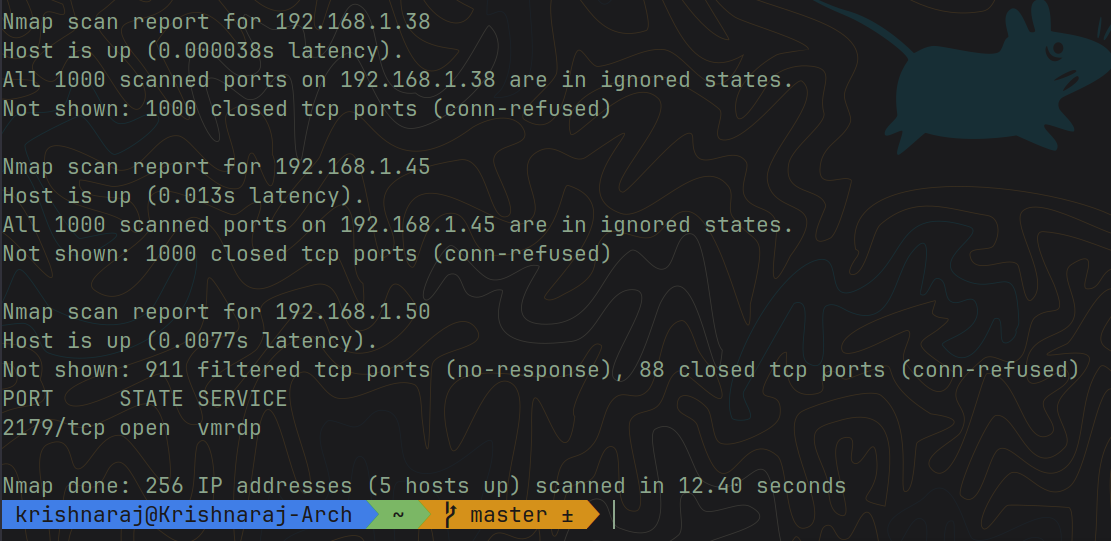
\includegraphics[width=0.8\textwidth]{scan ip range 2.png}
    \caption{scan range of ips. }
    \label{fig:1}
\end{figure}

\subsection{Scan 1 Port}

\subsubsection{Syntax}
\begin{verbatim}
$ nmap -p <port> <ip>
\end{verbatim}

\subsubsection*{Command}
\begin{verbatim}
$ nmap -p 80 www.example.com
\end{verbatim}

\subsubsection*{Purpose}
To perform a scan on a single port.

\subsubsection*{Output}
\begin{figure}[H]
    \centering
    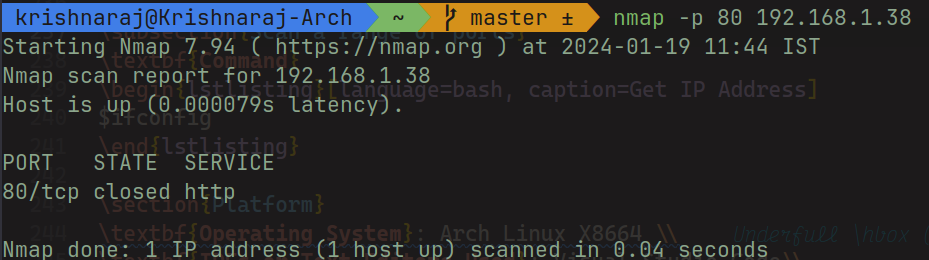
\includegraphics[width=0.8\textwidth]{nmap single port.png}
    \caption{Scan a single port}
    \label{fig:1}
\end{figure}

\subsection{Scan a range of ports}

\subsubsection{Syntax}
\begin{verbatim}
$ nmap -p <port range> <ip>
\end{verbatim}

\subsubsection*{Command}
\begin{verbatim}
$ nmap -p 1-100 www.example.com
\end{verbatim}

\subsubsection*{Purpose}
To perform a scan on a range of ports.

\subsubsection*{Output}
\begin{figure}[H]
    \centering
    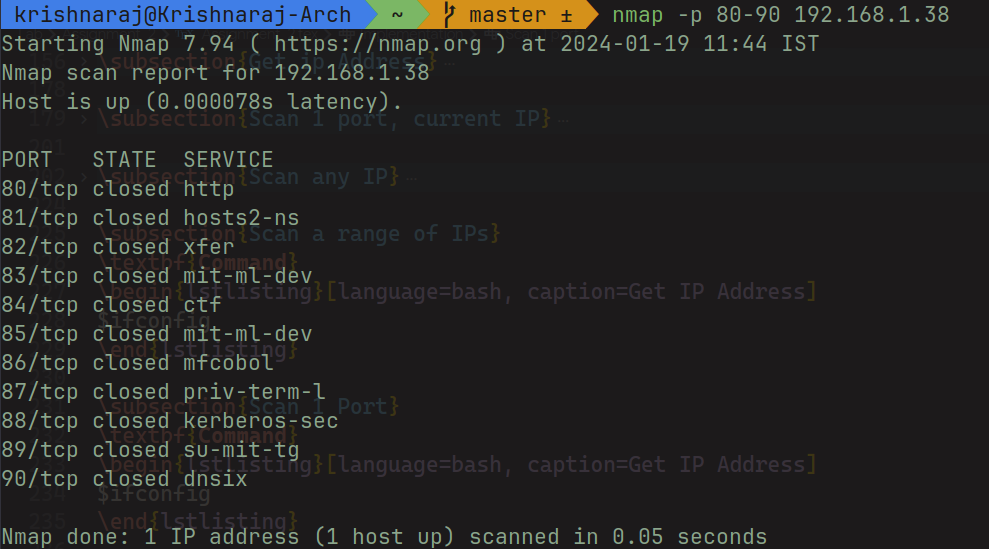
\includegraphics[width=0.8\textwidth]{nmap range of ports.png}
    \caption{Scan a range of ports}
    \label{fig:1}
\end{figure}

\subsection{Fragmented Scan}

\subsubsection{Syntax}
\begin{verbatim}
$ nmap -F <ip>
\end{verbatim}

\subsubsection*{Command}
\begin{verbatim}
$ nmap -F www.example.com
\end{verbatim}

\subsubsection*{Purpose}
Fragmented Scan is used to evade firewalls.

\subsubsection*{Output}
\begin{figure}[H]
    \centering
    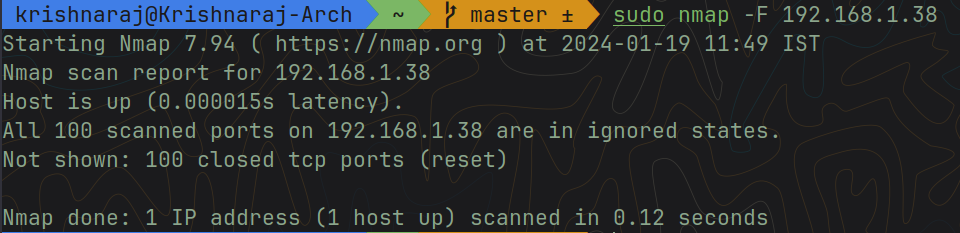
\includegraphics[width=0.8\textwidth]{nmap fragmented scan of 100 common ports.png}
    \caption{Perform a fragmented scan. }
    \label{fig:1}
\end{figure}

\subsection{TCP SYN Scan}

\subsubsection{Syntax}
\begin{verbatim}
$ nmap -sS <ip>
\end{verbatim}

\subsubsection*{Command}
\begin{verbatim}
$ nmap -sS www.example.com
\end{verbatim}

\subsubsection*{Purpose}
To scan a host for open ports using TCP SYN scan.

\subsubsection*{Output}
\begin{figure}[H]
    \centering
    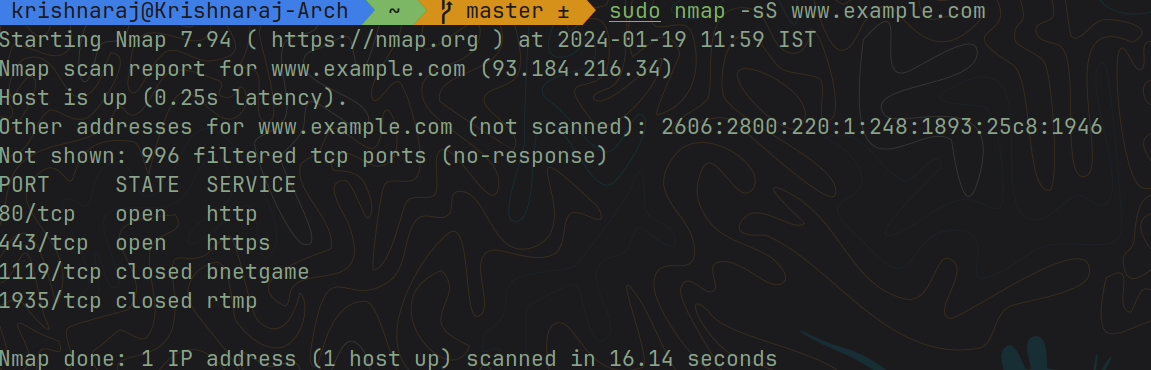
\includegraphics[width=0.8\textwidth]{nmap tcp syn.png}
    \caption{Check if tcp syn scan is possible on a host. }
    \label{fig:1}
\end{figure}

\subsection{OS Detection}

\subsubsection{Syntax}
\begin{verbatim}
$ nmap -O <ip>
\end{verbatim}

\subsubsection*{Command}
\begin{verbatim}
$ nmap -O www.example.com
\end{verbatim}

\subsubsection*{Purpose}
To scan operating system of a host.

\subsubsection*{Output}
\begin{figure}[H]
    \centering
    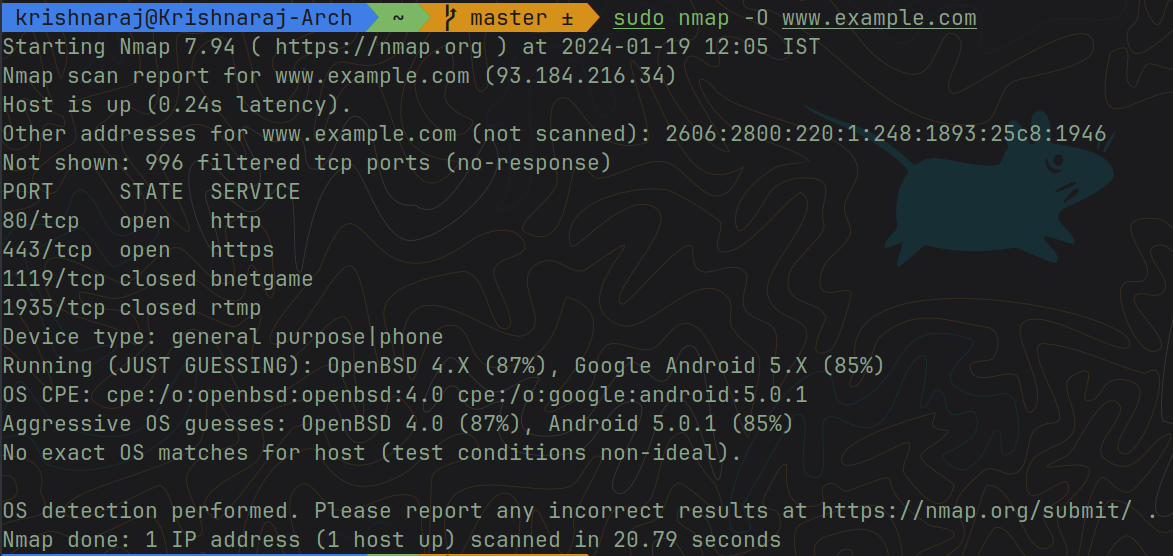
\includegraphics[width=0.8\textwidth]{nmap example os.png}
    \caption{Scan Operating System of example.com}
    \label{fig:1}
\end{figure}

\begin{figure}[H]
    \centering
    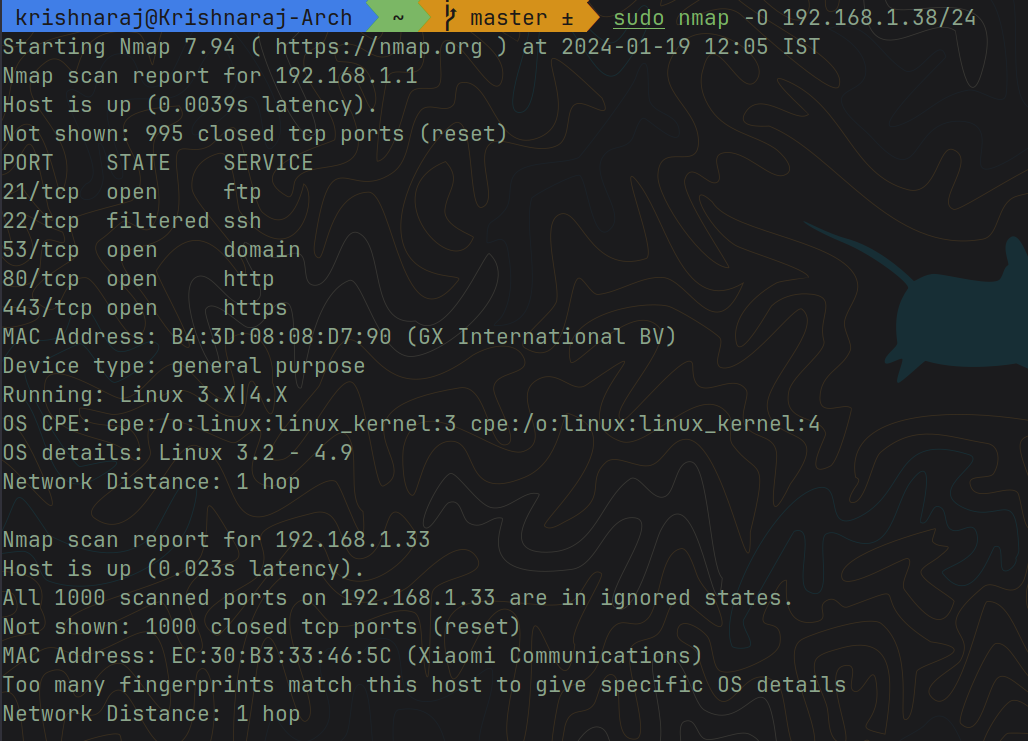
\includegraphics[width=0.8\textwidth]{nmap os host.png}
    \caption{Scan Operating System of host}
    \label{fig:1}
\end{figure}

\subsection{Syn Scan for specific ports with ping}
\subsubsection{Syntax}
\begin{verbatim}
$ sudo nmap -sS -p< <ip>
\end{verbatim}

\subsubsection*{Command}
\begin{verbatim}
$ sudo nmap -sS -p80-90 172.16.182.162
\end{verbatim}

\subsubsection*{Purpose}
To perform a syn scan on specific ports with ping.

\subsubsection*{Output}
\begin{figure}[H]
    \centering
    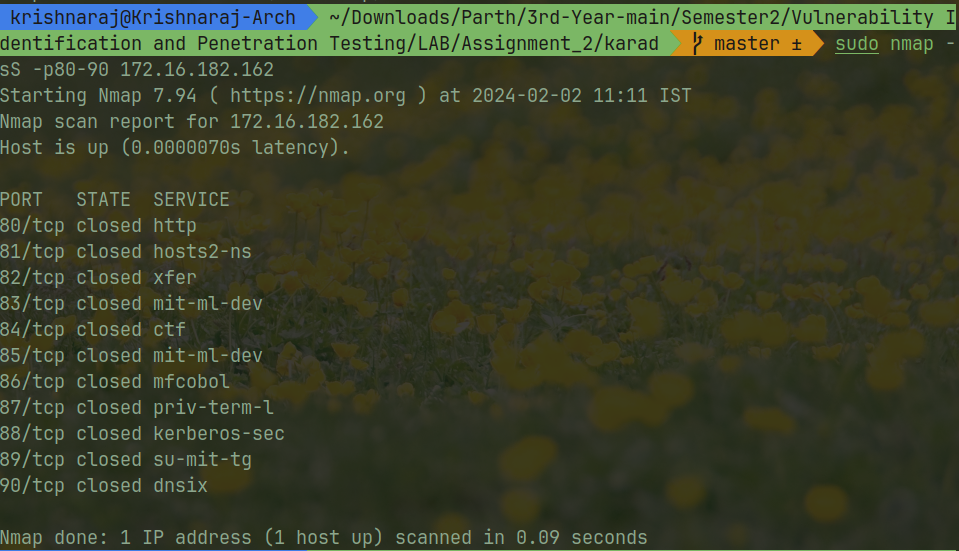
\includegraphics[width=0.8\textwidth]{with ping scan.png}
    \caption{scan with ping}
    \label{fig:1}
\end{figure}


\subsection{Syn Scan for specific ports without ping}
\subsubsection{Syntax}
\begin{verbatim}
$ sudo nmap -sS -Pn -p<port or range> <ip>
\end{verbatim}

\subsubsection*{Command}
\begin{verbatim}
$ sudo nmap -sS -Pn -p40-6000 172.16.182.162
\end{verbatim}

\subsubsection*{Purpose}
To scan the open ports of a host without ping to reduce time.

What is the use of ports from 80 to 90?

\begin{enumerate}
    \item \textbf{Port 80:} HTTP (Hypertext Transfer Protocol): Standard port used for serving web pages over the internet.
    \item \textbf{Port 81:} Alternative HTTP: Sometimes used as an alternative to port 80 for serving HTTP traffic.
    \item \textbf{Port 82:} Reserved: Not assigned for any specific use by the IANA.
    \item \textbf{Port 83:} Reserved: Not officially assigned for any specific use.
    \item \textbf{Port 84:} Commonly Unassigned: Doesn't have a well-known or standardized use.
    \item \textbf{Port 85:} Commonly Unassigned: No specific use assigned.
    \item \textbf{Port 86:} Commonly Unassigned: Typically not assigned.
    \item \textbf{Port 87:} Commonly Unassigned: Not typically used for any specific purpose.
    \item \textbf{Port 88:} Kerberos: Used by the Kerberos authentication system.
    \item \textbf{Port 89:} Commonly Unassigned: No well-known or standardized use.
\end{enumerate}


\subsubsection*{Output}
\begin{figure}[H]
    \centering
    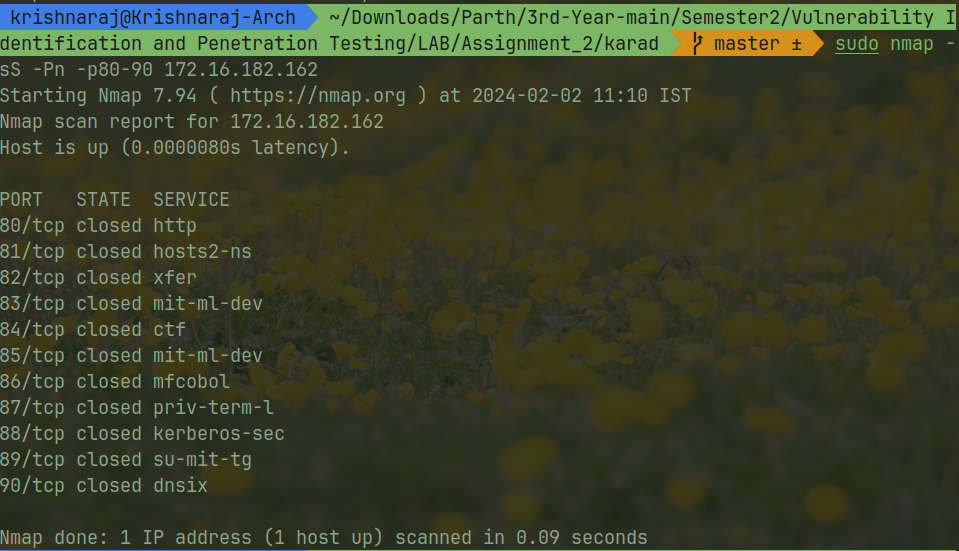
\includegraphics[width=0.8\textwidth]{without ping scan.png}
    \caption{scan without ping}
    \label{fig:1}
\end{figure}


\subsection{Nmap Timing Templates}

\begin{figure}[H]
    \centering
    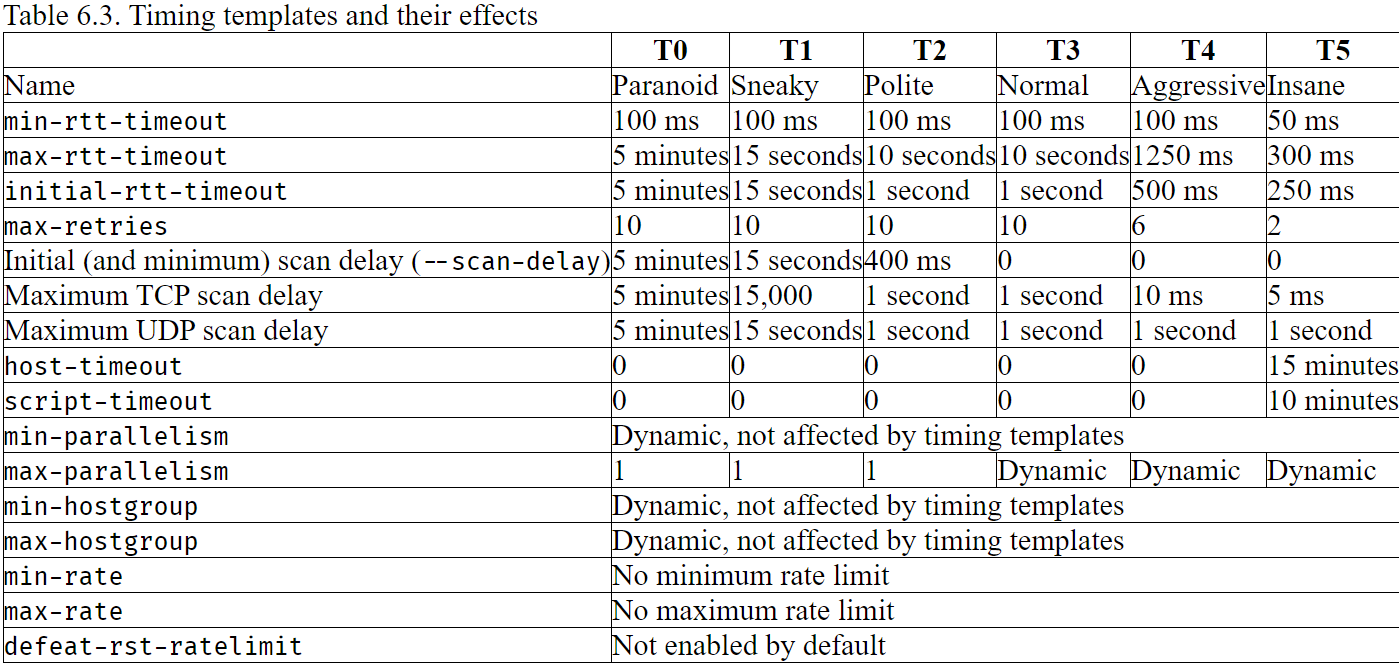
\includegraphics[width=.95\textwidth]{timing templates.png}
    \caption{}
\end{figure}

The use of these timing templates is to control the speed of the scan.\\
From the nmap documentation:

\begin{quotation}
    While the fine-grained timing controls discussed in the previous section are powerful and effective, some people find them confusing. Moreover, choosing the appropriate values can sometimes take more time than the scan you are trying to optimize. So Nmap offers a simpler approach, with six timing templates. You can specify them with the -T option and their number (0–5) or their name. The template names are paranoid (0), sneaky (1), polite (2), normal (3), aggressive (4), and insane (5). The first two are for IDS evasion. Polite mode slows down the scan to use less bandwidth and target machine resources. Normal mode is the default and so -T3 does nothing. Aggressive mode speeds scans up by making the assumption that you are on a reasonably fast and reliable network. Finally insane mode assumes that you are on an extraordinarily fast network or are willing to sacrifice some accuracy for speed.
\end{quotation}
    

\subsubsection{Syntax}
\begin{verbatim}
$ sudo nmap --packet-trace <ip> -T<0-6>
\end{verbatim}

\subsubsection*{Command}
\begin{verbatim}
$ sudo nmap --packet-trace antibrutus.surge.sh -T5
\end{verbatim}

\subsubsection*{Purpose}
To perform packet tracing with timing templates.

\subsubsection*{Output}
\begin{figure}[H]
    \centering
    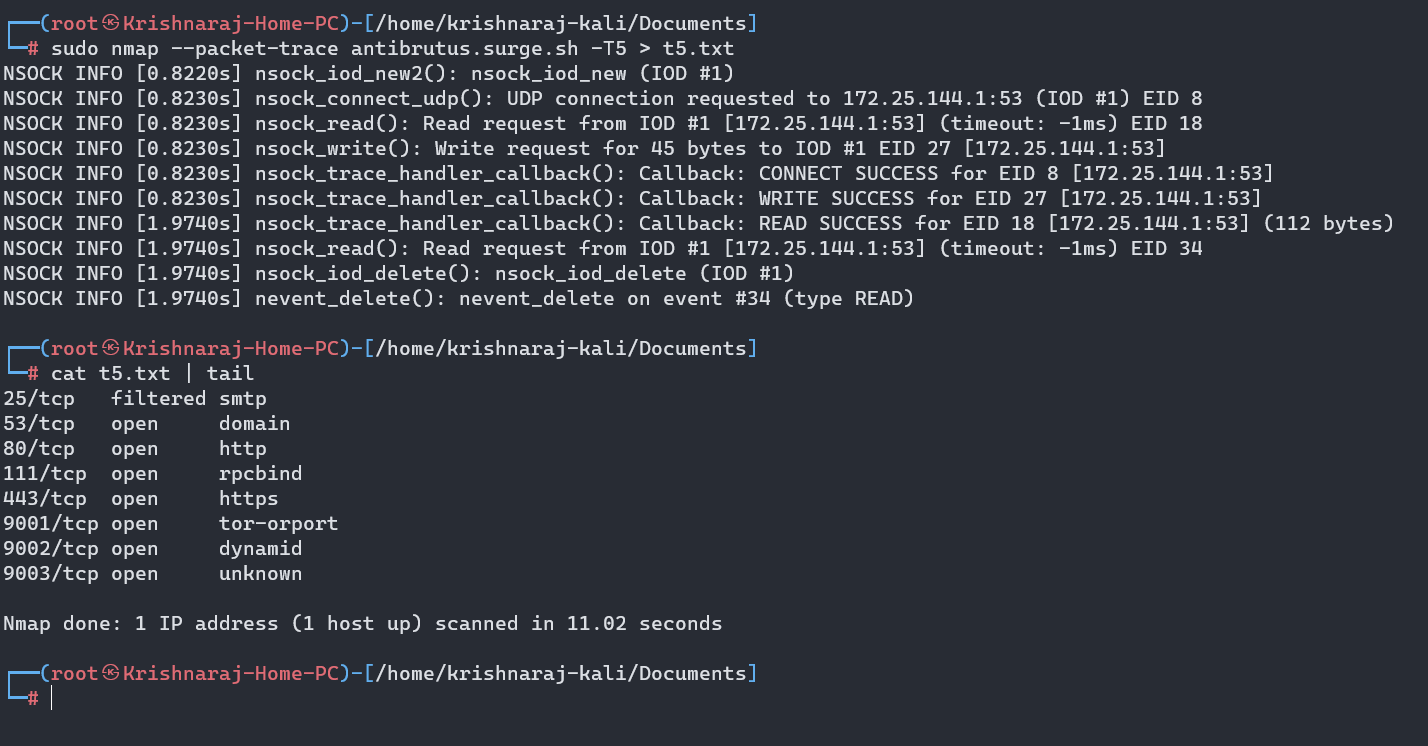
\includegraphics[width=0.9\textwidth]{t5.png}
    \caption{With T5}
    \label{fig:1}
\end{figure}
\begin{figure}[H]
    \centering
    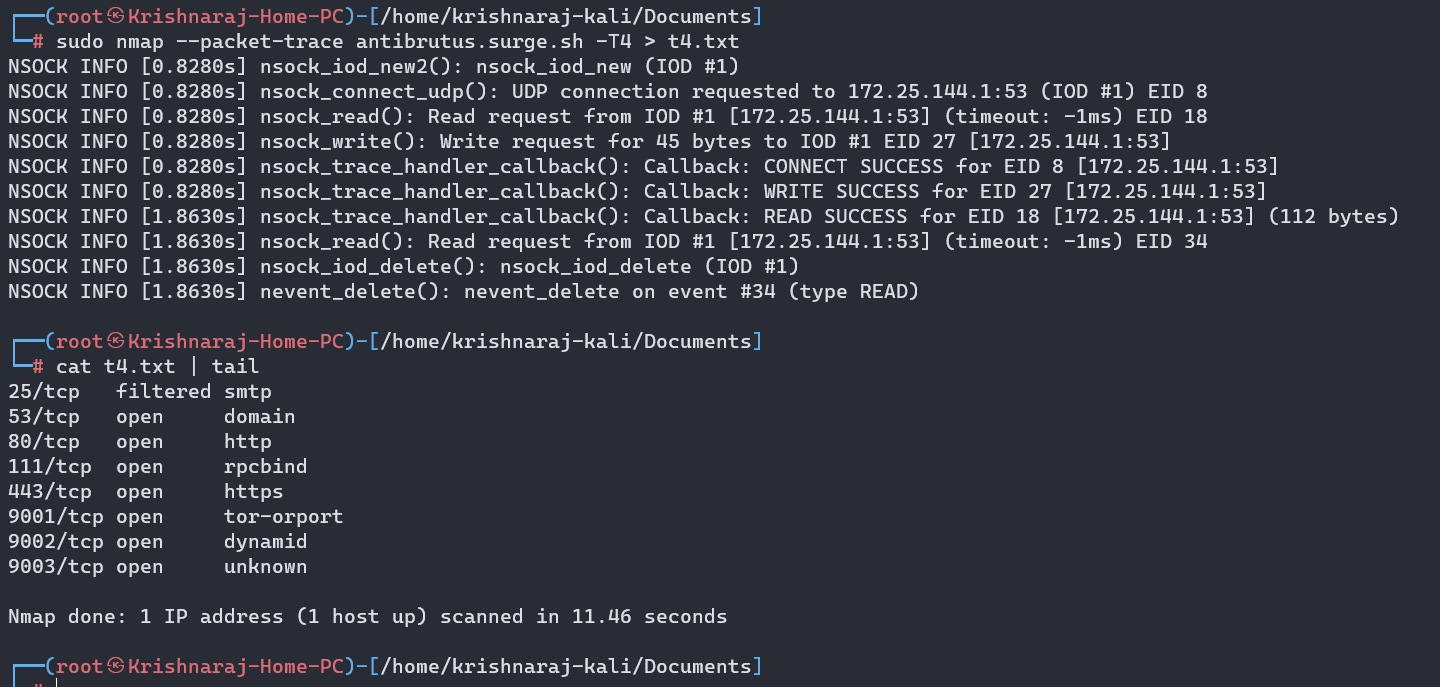
\includegraphics[width=0.9\textwidth]{t4.png}
    \caption{With T4}
    \label{fig:1}
\end{figure}
\begin{figure}[H]
    \centering
    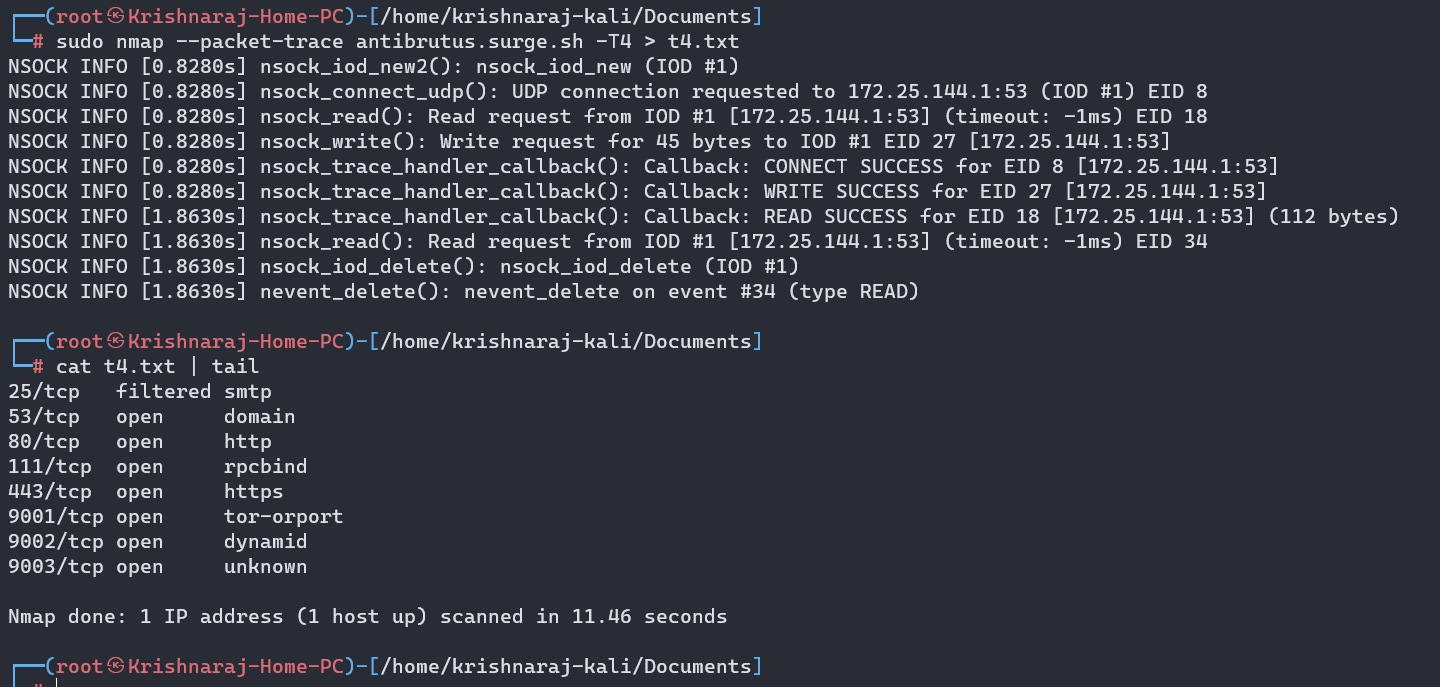
\includegraphics[width=0.9\textwidth]{t3.png}
    \caption{With T3}
    \label{fig:1}
\end{figure}
\begin{figure}[H]
    \centering
    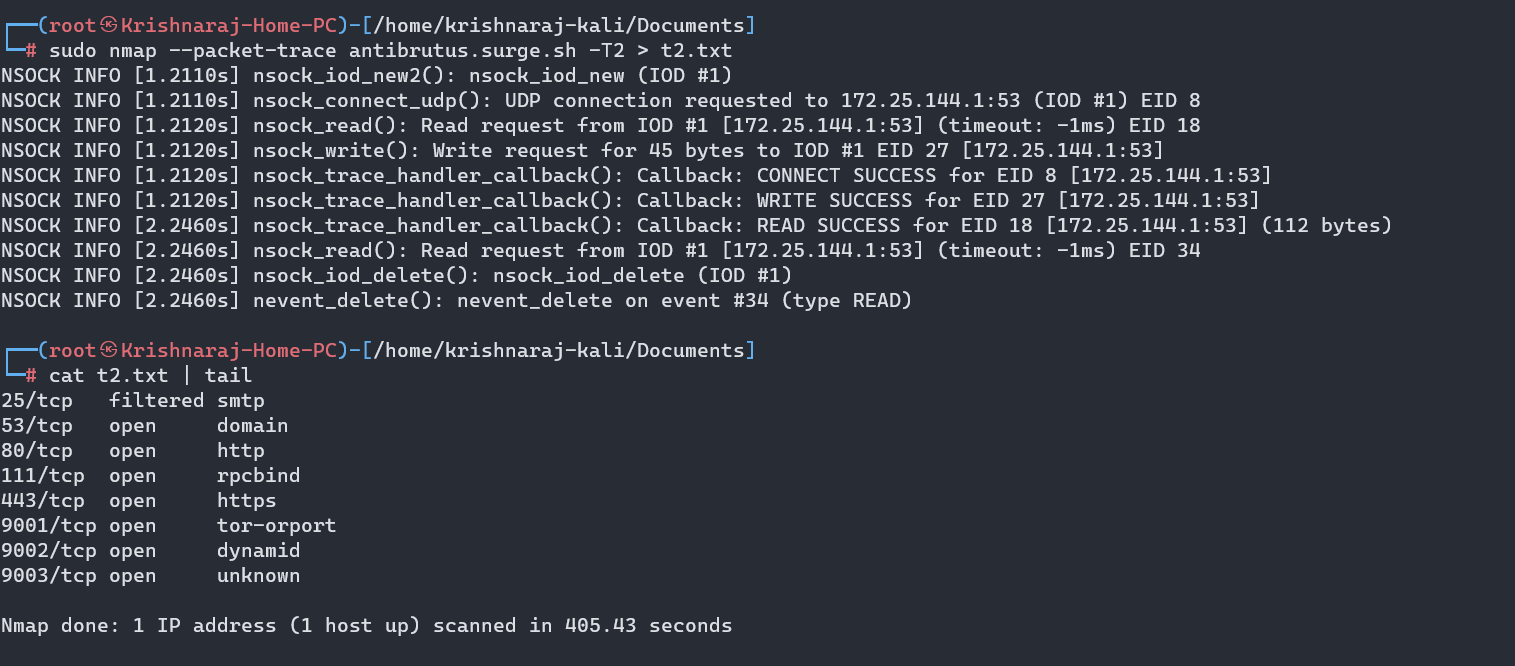
\includegraphics[width=0.9\textwidth]{t2.png}
    \caption{With T2}
    \label{fig:1}
\end{figure}

As we can see, the time taken per scan increases as we go from T5 to T2.


\subsection{Scannig Vulnerabilities}
\subsubsection{Syntax}
\begin{verbatim}
$ sudo nmap -Pn --script vuln <ip> -v
\end{verbatim}

\subsubsection*{Command}
\begin{verbatim}
$ sudo nmap -Pn --script vuln www.antibrutus.surge.sh -v
\end{verbatim}

\subsubsection*{Purpose}
To scan for vulnerabilities in a host.

\subsubsection*{Output}
\begin{figure}[H]
    \centering
    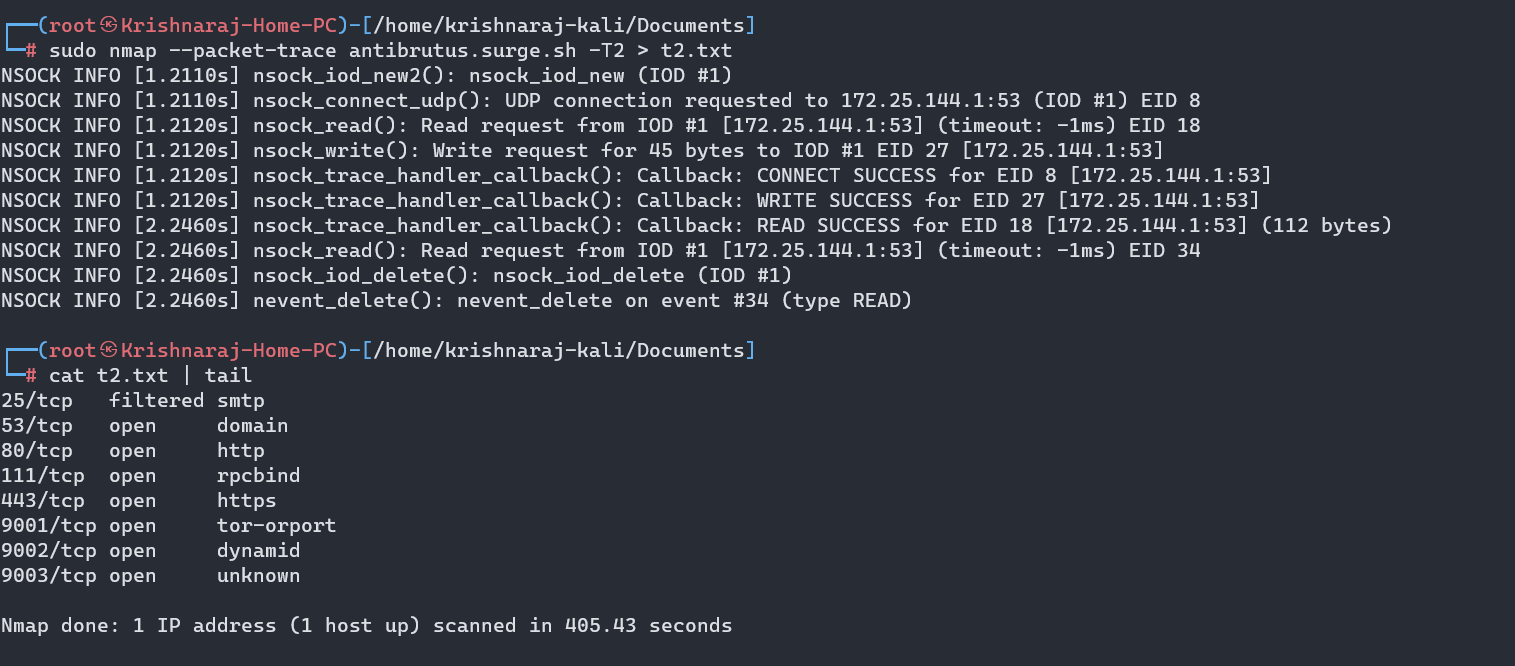
\includegraphics[width=0.9\textwidth]{vuln.png}
    \caption{Scan for vulnerabilities}
    \label{fig:1}
\end{figure}
\begin{figure}[H]
    \centering
    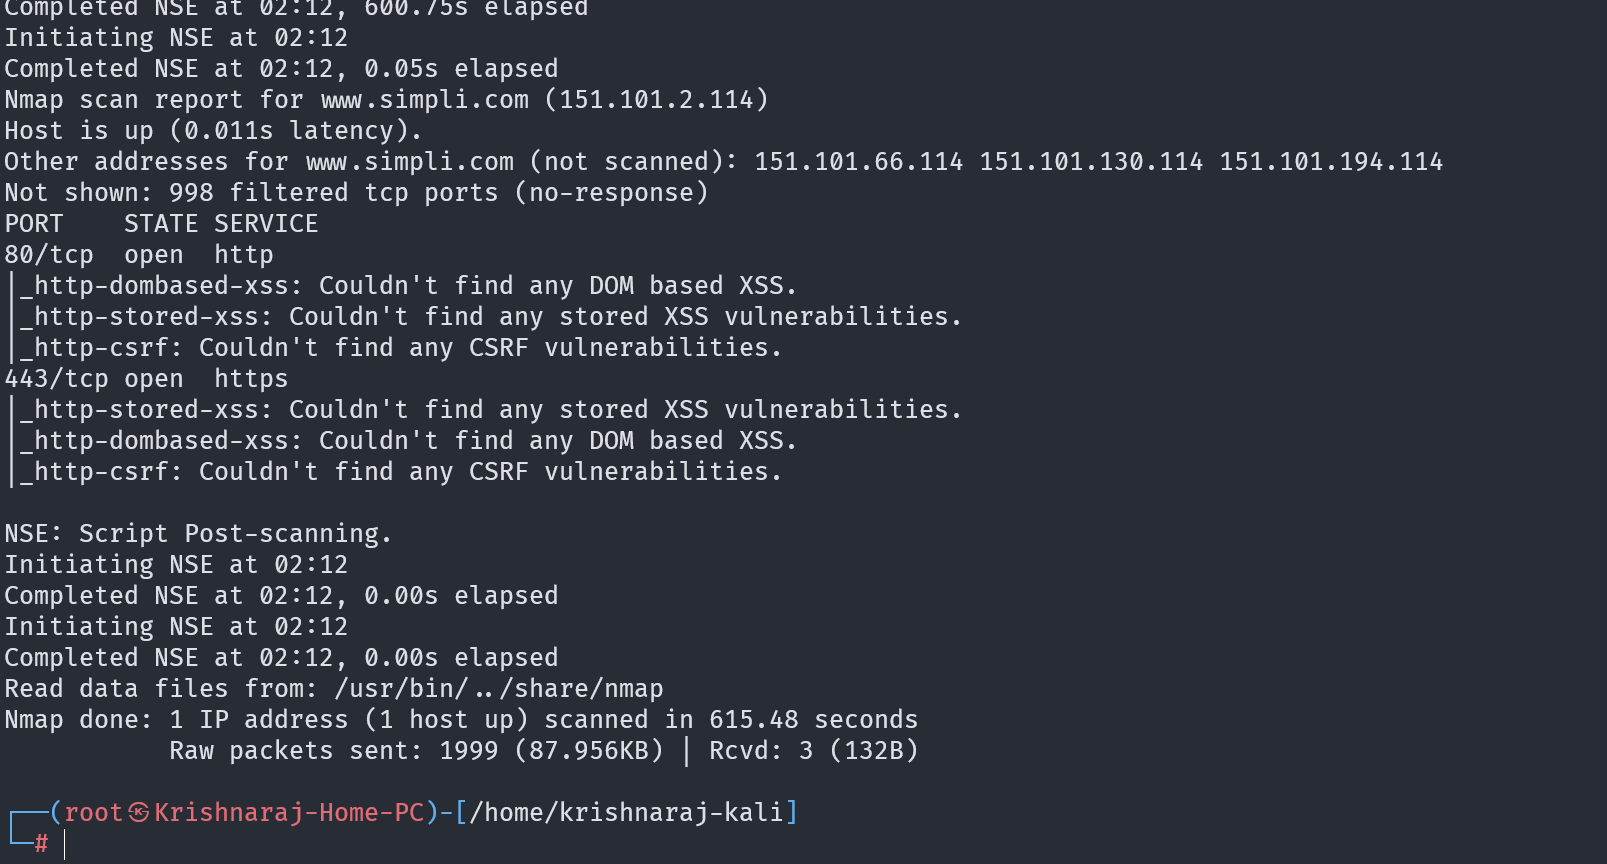
\includegraphics[width=0.9\textwidth]{vuln 2.png}
    \caption{Scan for vulnerabilities}
    \label{fig:1}
\end{figure}


\subsection*{Meaning of Scanned Vulnerabilities and Output}
\subsection*{Host Status}
\begin{itemize}
    \item \textbf{Host is up (0.011s latency):} Indicates that the host (www.simpli.com in this case) is up and responsive with a latency of 0.011 seconds.
\end{itemize}

\subsection*{Scanned Ports}
\begin{itemize}
    \item \textbf{80/tcp  open  http:} Port 80 is open and running an HTTP service, typically used for serving web pages.
    \item \textbf{443/tcp open  https:} Port 443 is open and running an HTTPS service, which is a secure version of HTTP.
\end{itemize}

\subsection*{Vulnerability Detection}

\subsubsection*{DOM-based XSS: DOM-based Cross-Site Scripting}

\textbf{Description:} DOM-based Cross-Site Scripting (XSS) is a type of XSS attack that occurs when an attacker injects malicious code into a web application, which is then executed by the victim's browser. The attack exploits vulnerabilities in the Document Object Model (DOM) of the web page to manipulate its content.

\subsubsection*{Stored XSS: Stored Cross-Site Scripting}

\textbf{Description:} Stored Cross-Site Scripting (XSS), also known as persistent XSS, occurs when an attacker injects malicious code into a web application, which is then stored and displayed to other users. The injected code is executed when other users visit the affected page, making it a serious security vulnerability.

\subsubsection*{CSRF: Cross-Site Request Forgery}

\textbf{Description:} Cross-Site Request Forgery (CSRF) is an attack that tricks a user into unknowingly executing unwanted actions on a web application in which they are authenticated. The attack occurs when an attacker exploits the user's active session to execute malicious requests without their consent. CSRF attacks can lead to unauthorized actions such as changing account settings or making financial transactions.

\subsection*{NSE Scripts}
\begin{itemize}
    \item NSE scripts were initiated and completed successfully, but no vulnerabilities were detected.
\end{itemize}

\subsection*{Scan Summary}
\begin{itemize}
    \item Nmap completed scanning 1 IP address with 1 host up in 615.48 seconds.
    \item 998 TCP ports were filtered (no response), and 2 ports were open (HTTP and HTTPS).
\end{itemize}



\subsection{Sweeping IP Ranges for Live host using ARP Scan}

\subsubsection{Syntax}
\begin{verbatim}
$ nmap -PR -sn <ip range>
\end{verbatim}

\subsubsection*{Command}
\begin{verbatim}
$ nmap -PR -sn 172.16.182.224/24
\end{verbatim}

\subsubsection*{Purpose}
To scan live hosts using ARP scan.

\subsubsection*{Output}
\begin{figure}[H]
    \centering
    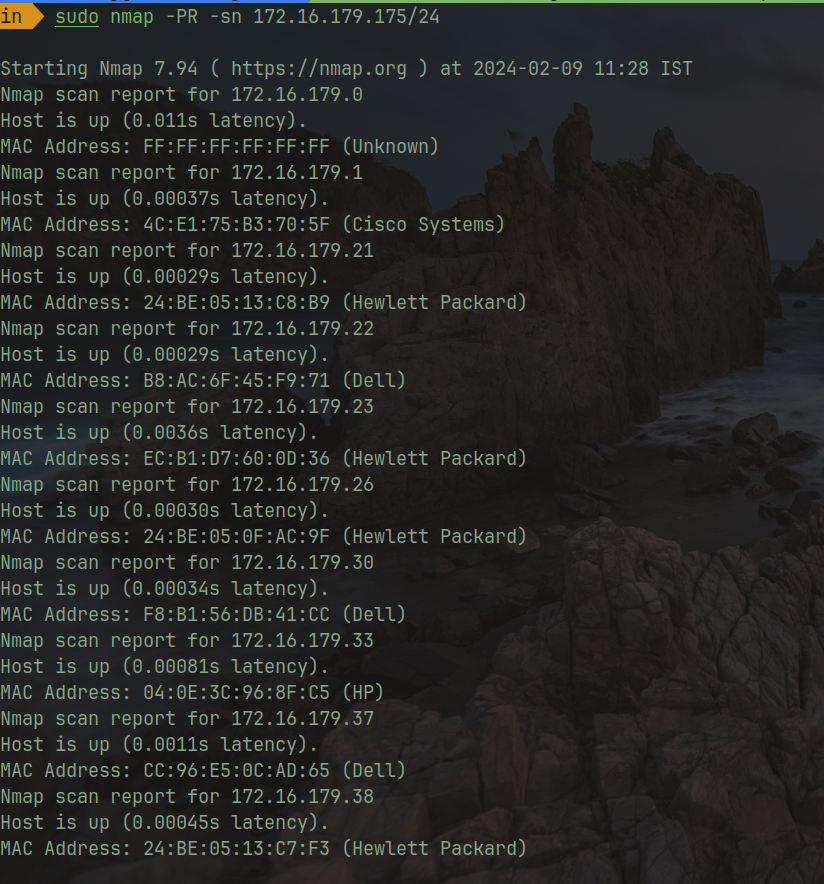
\includegraphics[width=0.8\textwidth]{arp scan.png}
    \caption{To scan live hosts using arp scan.}
    \label{fig:1}
\end{figure}


\subsection{Sweeping IP Ranges for Live host using ICMP Scan}

\subsubsection{Syntax}
\begin{verbatim}
$ nmap -PP -sn <ip range>
\end{verbatim}

\subsubsection*{Command}
\begin{verbatim}
$ nmap -PP -sn 172.16.182.224
\end{verbatim}

\subsubsection*{Purpose}
To scan live hosts using ICMP scan.

\subsubsection*{Output}
\begin{figure}[H]
    \centering
    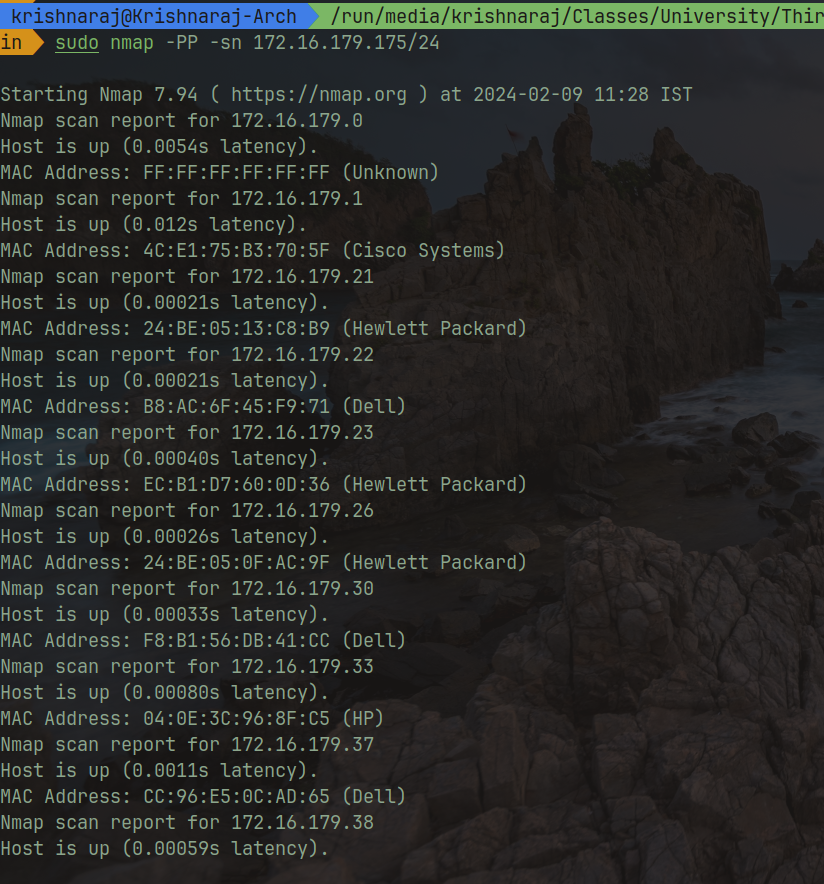
\includegraphics[width=0.8\textwidth]{icmp scan.png}
    \caption{To scan live hosts using ICMP scan.}
    \label{fig:1}
\end{figure}

\subsection{Sweeping IP Ranges for Live host using TCP Scan}

\subsubsection{Syntax}
\begin{verbatim}
$ nmap -PA -sn <ip range>
\end{verbatim}

\subsubsection*{Command}
\begin{verbatim}
$ nmap -PA -sn 172.16.182.224
\end{verbatim}

\subsubsection*{Purpose}
To scan live hosts using TCP scan. This performs 3 way handshaking as opposed to the -sS syn scan option which does not perform 3 way handshaking.

\subsubsection*{Output}
\begin{figure}[H]
    \centering
    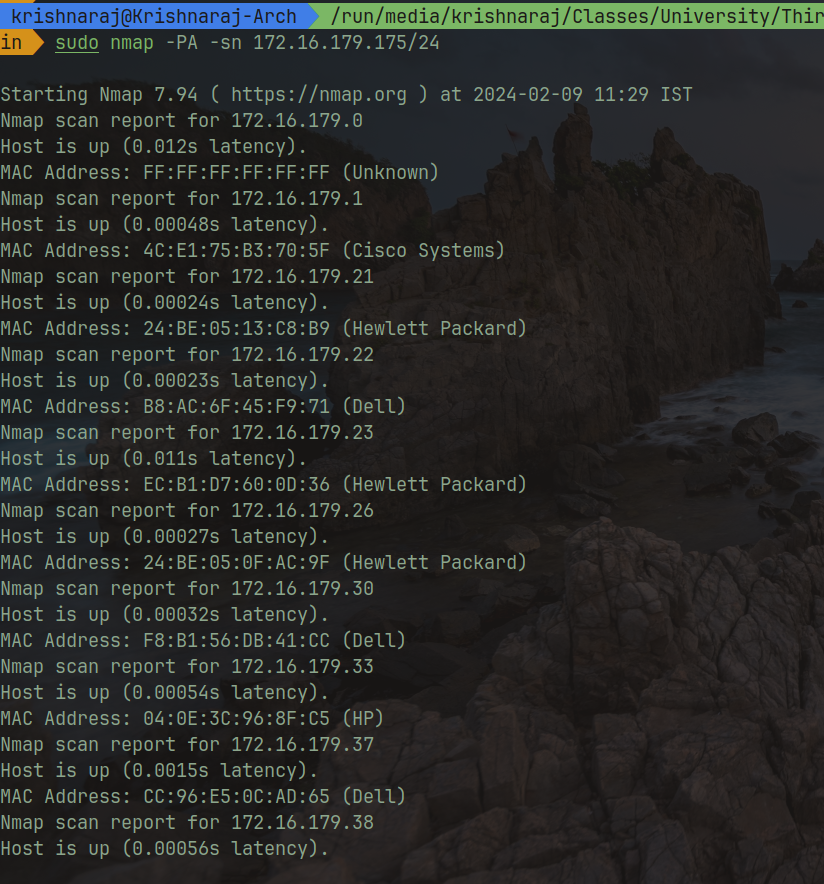
\includegraphics[width=0.8\textwidth]{tcp scan.png}
    \caption{To scan live hosts using TCP scan.}
    \label{fig:1}
\end{figure}


\subsection{Sweeping IP Ranges for Live host using UDP Scan}

\subsubsection{Syntax}
\begin{verbatim}
$ nmap -PU -sn <ip range>
\end{verbatim}

\subsubsection*{Command}
\begin{verbatim}
$ nmap -PU -sn 172.16.182.224
\end{verbatim}

\subsubsection*{Purpose}
To scan live hosts using UDP scan.

\subsubsection*{Output}
\begin{figure}[H]
    \centering
    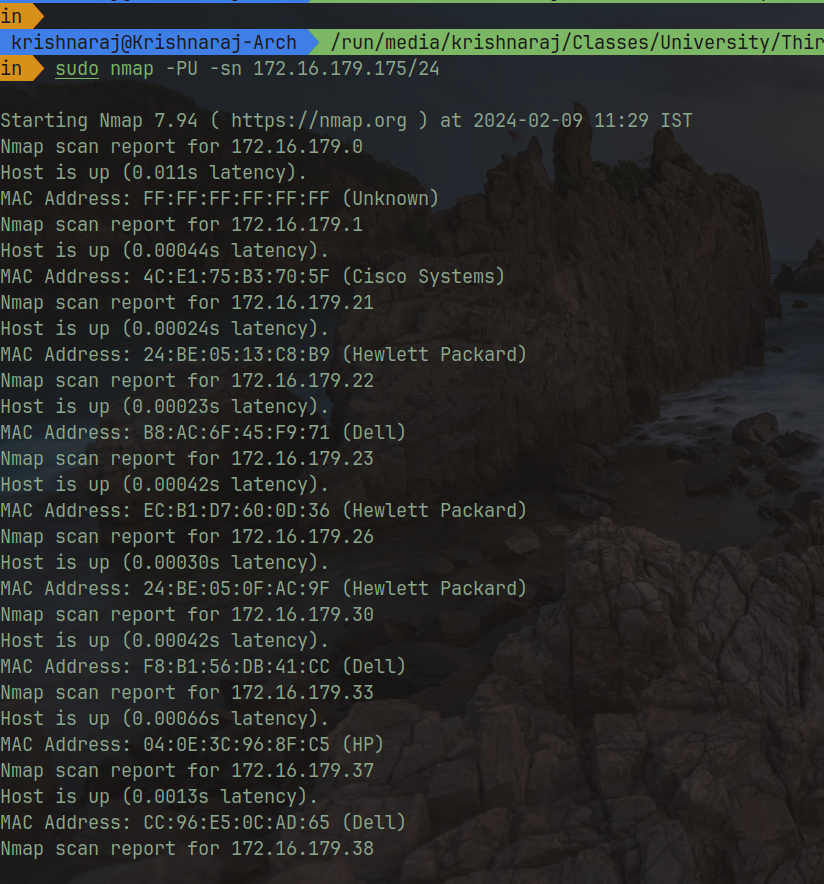
\includegraphics[width=0.8\textwidth]{udp scan.png}
    \caption{To scan live hosts using UDP scan.}
    \label{fig:1}
\end{figure}


\clearpage
\begin{thebibliography}{99}
	\bibitem{wireshark}
	Wireshark. \\
	Website: \url{https://www.wireshark.org/}

	\bibitem{tshark}
	Tshark. \\
	Website: \url{https://www.wireshark.org/docs/man-pages/tshark.html}

	\bibitem{tcpdump}
	Tcpdump. \\
	Website: \url{https://www.tcpdump.org/}

	\bibitem{aircrack}
	AirCrack-ng. \\
	Website: \url{https://www.aircrack-ng.org/}

	\bibitem{airsnort}
	AirSnort. \\
	Website: \url{https://sourceforge.net/projects/airsnort/}
\end{thebibliography}

\end{document}